\documentclass[10pt,a4paper]{article}
\usepackage[utf8]{inputenc}
\usepackage[italian]{babel}
\usepackage{amsmath}
\usepackage{amsfonts}
\usepackage{amssymb}
\usepackage{graphicx}
\usepackage{siunitx}
\usepackage{textcomp}
\usepackage[left=2cm,right=2cm,top=2cm,bottom=2cm]{geometry}
\newcommand{\rem}[1]{[\emph{#1}]}
\newcommand{\exn}{\phantom{xxx}}
\renewcommand{\thesubsection}{\thesection.\alph{subsection}} 
\renewcommand{\thesubsubsection}{\thesection.\alph{subsection}.\alph{subsubsection}}

\title{Esperienza di Franck-Hertz con Neon}
\author{Fabrizio Chicconi, Lorenzo Cavuoti, Simone Antognetti}
\date{4 Aprile 2019}

\begin{document}

\maketitle


\section*{Introduzione}
L'obiettivo di questa esperienza è quello di osservare gli effetti dovuti alla struttura discreta dei livelli energetici dell'atomo di Neon e di stimare la separazione fra lo stato fondamentale ed il primo gruppo di stati eccitati.

\section{Materiale utilizzato}
L'esperienza è stata svolta utilizzando la seguente strumentazione:
\begin{itemize}
\item Tetrodo a gas Neon ELWE U8482230;
\item Sistema di alimentazione e di misura di corrente ELWE;
\item Oscilloscopio.
\end{itemize}

\section{Descrizione dell'apparato sperimentale}
In Fig.~\ref{fig:schema} si può osservare lo schema dell'apparato sperimentale.
\begin{figure}[h!]
	\centering
	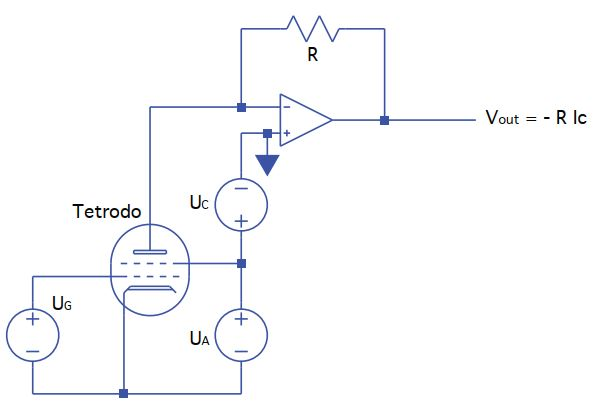
\includegraphics[scale=0.7]{schema}
	\caption{Schema dell'apparato sperimentale}
	\label{fig:schema}
\end{figure}
Il Tetrodon è un tubo elettronico a gas riempito di Neon in cui sono presenti quattro elettrodi. Il catodo nella parte inferiore viene riscaldato ed è responsabile dell'emissione di elettroni, a bassa energia rispetto alle altre in gioco ($\sim$0.1 eV), per effetto termoionico.

Sono presenti in ordine del basso la griglia di controllo e la griglia anodo, entrambe costituite da una fitta rete di sottili fili conduttori, che sono praticamente trasparenti agli elettroni che devono passare, ma abbastanza fitte da poter essere considerate un piano equipotenziale dal punto di vista elettrostatico.

Infine nella parte superiore è presente il collettore, un conduttore piano che raccoglie gli elettroni che giungono sulla sua superficie.

\newpage
Il generatore utilizzato nell'esperienza applica le seguenti tensioni agli elettrodi come mostrato in Fig.~\ref{fig:schema}:
\begin{itemize}
\item U\ped{F} è la tensione applicata al filamento che scalda il catodo e ne regola la temperatura regolando di conseguenza l'emissione di elettroni;
\item U\ped{G} è la tensione applicata fra griglia di controllo e catodo utile ad aumentare l'emissività;
\item U\ped{A} è la differenza di potenziale applicata fra catodo e griglia anodo allo scopo di accelerare gli elettroni emessi verso il collettore;
\item U\ped{E} è la differenza di potenziale applicata fra griglia anodo e collettore allo scopo di frenare gli elettroni che superato l'anodo siano diretti verso l'elettrodo di raccolta.
\end{itemize}
Infine il collettore è collegato ad una transimpedenza che fornisce un segnale in tensione proporzionale alla corrente in uscita dal collettore I\ped{C}.

%PIù o meno da queste parti inserirei una brevissima sezione dove si spiega il fenomeno dell'eccitazione del Neon, così da darlo per scontato nel resto della relazione, cosa ne pensate?

\section{Osservazioni ed interpretazioni}
In questa fase dell'esperienza si procede all'accensione dell'apparato come da procedura indicata sulla nota di accompagnamento e si fanno osservazioni e misure della struttura luminosa all'interno del tetrodo al variare di U\ped{F}, U\ped{G}, U\ped{A} ed U\ped{E}, fornendone un interpretazione fenomenologica.

\subsection*{Struttura luminosa al variare di U\ped{A} e U\ped{G}}
Variando le tensioni U\ped{A} e U\ped{G} si osserva una sostanziale modifca della struttura luminosa all'interno del tetrodo. 

\subsubsection*{Variazione di U\ped{A}}
Partendo da valori piccoli di U\ped{A} e aumentandoli si osserva:
\begin{itemize}
\item [] \textbf{spostamento delle bande verso la griglia di controllo} può essere spiegato tenendo in considerazione che aumentando il valore di U\ped{A} gli elettorni vengo maggiormente accelerati e dunque raggiungeranno in uno spazio minore l'energia cinetica necessaria a compiere urti anelastici che eccitino gli atomi di Neon, determinando dunque lo spostamento osservato; 
\item [] \textbf{comparsa di nuove bande} come nel punto precedente grazie alla maggior accelerazione gli elettroni riescono a raggiungere a parità di spazio energie più alte e dunque a portare tramite gli urti il Neon a stati di eccitazione con energie via via crescenti salendo nelle bande;
\item [] \textbf{variazione di luminosità e deformazione} %qui sono un po' incerto su cosa dire, effetti al bordo? Più elettroni collidono?  Perché più elettroni collidono?
\end{itemize}
\subsubsection*{Variazione di U\ped{G}}
Partendo da valori piccoli e aumentandoli si osserva:
\begin{itemize}
\item [] \textbf{aumento di luminosità delle bande} dovuto al fatto che l'aumentare di U\ped{G} fa si che più elettroni vengano estratti per effetto termoionico dal catodo determinando così un numero maggiore di elettroni che collidendo porterano il Neon nei vari stati eccitati;
\item [] \textbf{deformazione delle bande} si osserva che le bande assumono una conformazione concava e si suppone sia dovuto ad un efffetto ai bordi, cioè ad una diversa accelerazione degli elettroni che si trovano più a ridosso delle pareti esterne del tetrodo.
\end{itemize}

\subsection*{Misure di U\ped{A}}
In questa fase dell'esperienza a turno abbiamo osservato all'interno del tetrodo quando comparivano le varie bande luminose al variare di U\ped{A} prendendone il valore dal generatore. La stima dell'incertezza è stata fatta non tenendo conto dell'incertezza sulla lettura dovuta al generatore che si è ritenuta trascurabile rispetto a quella dovuta alla difficoltà di individuare esattamente quando comparissero le varie bande luminose. %%Il discorso sugli errori poi vediamo di chiarirlo meglio 
I valori ottenuti sono riassunti in Tabella~\ref{tab:ua}. \newpage
\begin{table}[h]
	\centering
	\caption{\small Valori di U\ped{A} per cui compaiono le bande luminose}
	\vspace{1mm}
	\begin{tabular}{cc}\hline
	& \textbf{U\ped{A} [V]} \\
	\hline\hline
	\textbf{Prima banda} & 25.5 $\pm$ xxx  \\
	\textbf{Seconda banda} & 41.2 $\pm$ xxx \\
	\textbf{Terza banda} & 55.2 $\pm$ xxx \\ \hline
	\end{tabular}
	\label{tab:ua}
\end{table}
%Ho solo brutalmente fatto la media delle nostre tre misure, con l'ovvio però che l'ultima è veramente molto incerta, prima dovremmo farci un'idea se almeno fossimo lontani o meno dai valori che avremmo dovuto osservare
\noindent Queste misurazioni possono fornire una prima stima grossolana dell'energia dei vari stati eccitati del Neon che si osservano nel tetrodo. Gli elettroni accelerati arrivano in porssimità dell'anodo con energia cinetica K = e$\cdot$U\ped{A}.

\subsection*{I\ped{C} vs U\ped{A} con U\ped{E} = 0V}

\end{document}